\section{Steady-state output ceilings and finite electrical demand}
\label{sec:freq}

Two driver limits bound steady sinusoidal output: linear excursion and
continuous coil dissipation. Both are established results
\cite{small1972direct}; they are restated here on the reference bases of
\cref{sec:scope-bases} so that the gates below are unambiguous.

\subsection{Displacement- and dissipation-limited ceilings}
\label{sec:freq-ceilings}

With $\Vd\equiv\Sd\Xmax$ (peak displaced volume) and
$\hat p_{\mathrm L}(\omega)=\rho_0\omega^2\Vd/(2\pi r)$, the
excursion-limited intrinsic ceiling (basis B1) is

\begin{equation}
	\boxed{\ \mathrm{SPL}_{\mathrm{L}}(f)=
			108.5+20\log_{10}\!\big(f^2\,\Vd\big)\ \mathrm{dB}\ }
	\label{eq:SPLL}
\end{equation}

(rms pressure, $r=\SI{1}{\meter}$, half space, $+12$\,dB/oct). It depends
on no other parameter: within this model $\Qtc$, $F_c$, $\Bl$, $\Re$,
$\Mms$, and $\Pmax$ do not appear, so in the excursion-limited regime
$\Vd$ alone orders candidates. The alignment governs corner placement,
settling, and the drive required to reach the ceiling, not the ceiling
itself.

With the reference efficiency

\begin{equation}
	\eta_0 =
		\frac{\rho_0}{2\pi c} \,
		\frac{\Bl^2\Sd^2}{\Re\Mms^2}
		= 9.78\times10^{-7}\ \frac{F_s^3\,\Vas[\mathrm{m^3}]}{\Qes},
	\label{eq:eta0}
\end{equation}

the dissipation-limited passband ceiling is

\begin{equation}
	\boxed{\ \mathrm{SPL}_{\mathrm{T}}=112.2+10\log_{10}\!\big(\eta_0\Pmax\big)\ \mathrm{dB}\ }
	\label{eq:SPLT}
\end{equation}

on the same basis, obtained by substituting $\hat\imath=\sqrt{2P/\Re}$ into
\cref{eq:iofx,eq:pofx}. The two ceilings combine as

\begin{equation}
	p_{\max}(\omega) =
		\frac{\rho_0\Sd\,\omega^2}{2\pi r}\;
		\min\!\Big\{\Xmax,\ X_{\mathrm{T}}(\omega)\Big\},
	\label{eq:master}
\end{equation}

and cross at

\begin{equation}
	f_x =
		\frac{1}{2\pi}\left(\frac{4\pi c\,\eta_0\Pmax}{\rho_0\,\Vd^{2}}\right)^{1/4} .
	\label{eq:fx}
\end{equation}

Below $f_x$ additional $\Vd$ raises the ceiling; above it additional
$\eta_0\Pmax$ does. These are \emph{ceilings}: adequacy is decided at the
target level of \cref{sec:room}, not at the ceiling, so a driver whose
regime boundary lies inside its band may still be far from either limit at
the declared target.

\subsection{Demand and finite amplifier gates}
\label{sec:freq-gates}

Let $V_{\mathrm{dem}}(f)$ be the peak displaced volume required at the
couch-area reference (basis B2--B4, \cref{sec:room}), and let the role be
served by $N$ identical drivers sharing one common signal (A9), so the
per-driver peak displacement is
$X_{\mathrm{dem}}(f)=V_{\mathrm{dem}}(f)/(N\Sd)$. Inverting
\cref{eq:xofe,eq:iofx} gives the exact steady requirements per physical
driver, in rms:

\begin{align}
	E_{\mathrm{req}}(\omega)&=
		\frac{\Re\Mms}{\sqrt2\,\Bl}\,X_{\mathrm{dem}}
		\sqrt{(\wc^2-\omega^2)^2+\sigma^2\omega^2},
		\label{eq:Ereq}\\
	I_{\mathrm{req}}(\omega)&=
		\frac{\Mms}{\sqrt2\,\Bl}\,X_{\mathrm{dem}}
		\sqrt{(\wc^2-\omega^2)^2+\sm^2\omega^2},
		\label{eq:Ireq}\\
	P_{\mathrm{req}}(\omega)&=
		\frac{\Mms\Qes X_{\mathrm{dem}}^{2}}{4\pi F_s}
		\Big[(\wc^2-\omega^2)^2+\sm^2\omega^2\Big] .
		\label{eq:Preq}
\end{align}

\Cref{eq:Preq} is a ``bathtub'' in $\omega$: minimum near $\wc$, finite at
DC, and rising both below the corner (the correction cost of holding a flat
target through the sealed roll-off, $12$\,dB/oct in power) and above it
(the $\omega^4$ growth of the pressure required from a fixed displacement).
Both branches must be evaluated across the complete role band, since the
worst voltage, worst current, and worst power generally occur at different
frequencies.

The feasibility gates are then, for every $f$ in the role band and for
every physical driver,
\begin{equation}
	\boxed{\
	\begin{aligned}
	E_{\mathrm{req}}&\le E_{\mathrm{amp}}, &
	I_{\mathrm{req}}&\le I_{\mathrm{amp}},\\
	E_{\mathrm{burst}}&\le E_{\mathrm{amp}}, &
	I_{\mathrm{burst}}&\le I_{\mathrm{amp}},\\
	P_{\mathrm{req}}&\le\min\{\Pmax,\ P_{\mathrm{amp,cont}}\}, &
	P_{\mathrm{burst}}&\le P_{\mathrm{amp,burst}},
	\end{aligned}\ }
	\label{eq:ampgates}
\end{equation}

with the burst quantities from \cref{sec:time}, together with
$\xi_x=X_{\mathrm{dem}}/\Xmax\le1$ (A7). A candidate failing any gate at
any frequency in its band is rejected, with the binding gate and frequency
recorded.

DSP correction is not free. Flattening the response below the corner
multiplies \cref{eq:Preq} by roughly $(\wc/\omega)^4$ and the required
displacement by $(\wc/\omega)^2$; it also raises current, coil temperature,
and---through the resulting rise in $\Re$ \cite{button1992}---detunes
$\Qtc$ and $F_c$ during sustained programme. Correction is therefore
applied over a finite band, and its cost is charged to
\cref{eq:Ereq,eq:Ireq,eq:Preq} rather than assumed away.
\Cref{fig:output-electrical} shows both sides of this check for both roles:
the margin of the combined ceiling \cref{eq:master} over the couch-area
target, and the resulting electrical demand against the declared limits.

\begin{figure}[htbp]
	\centering
	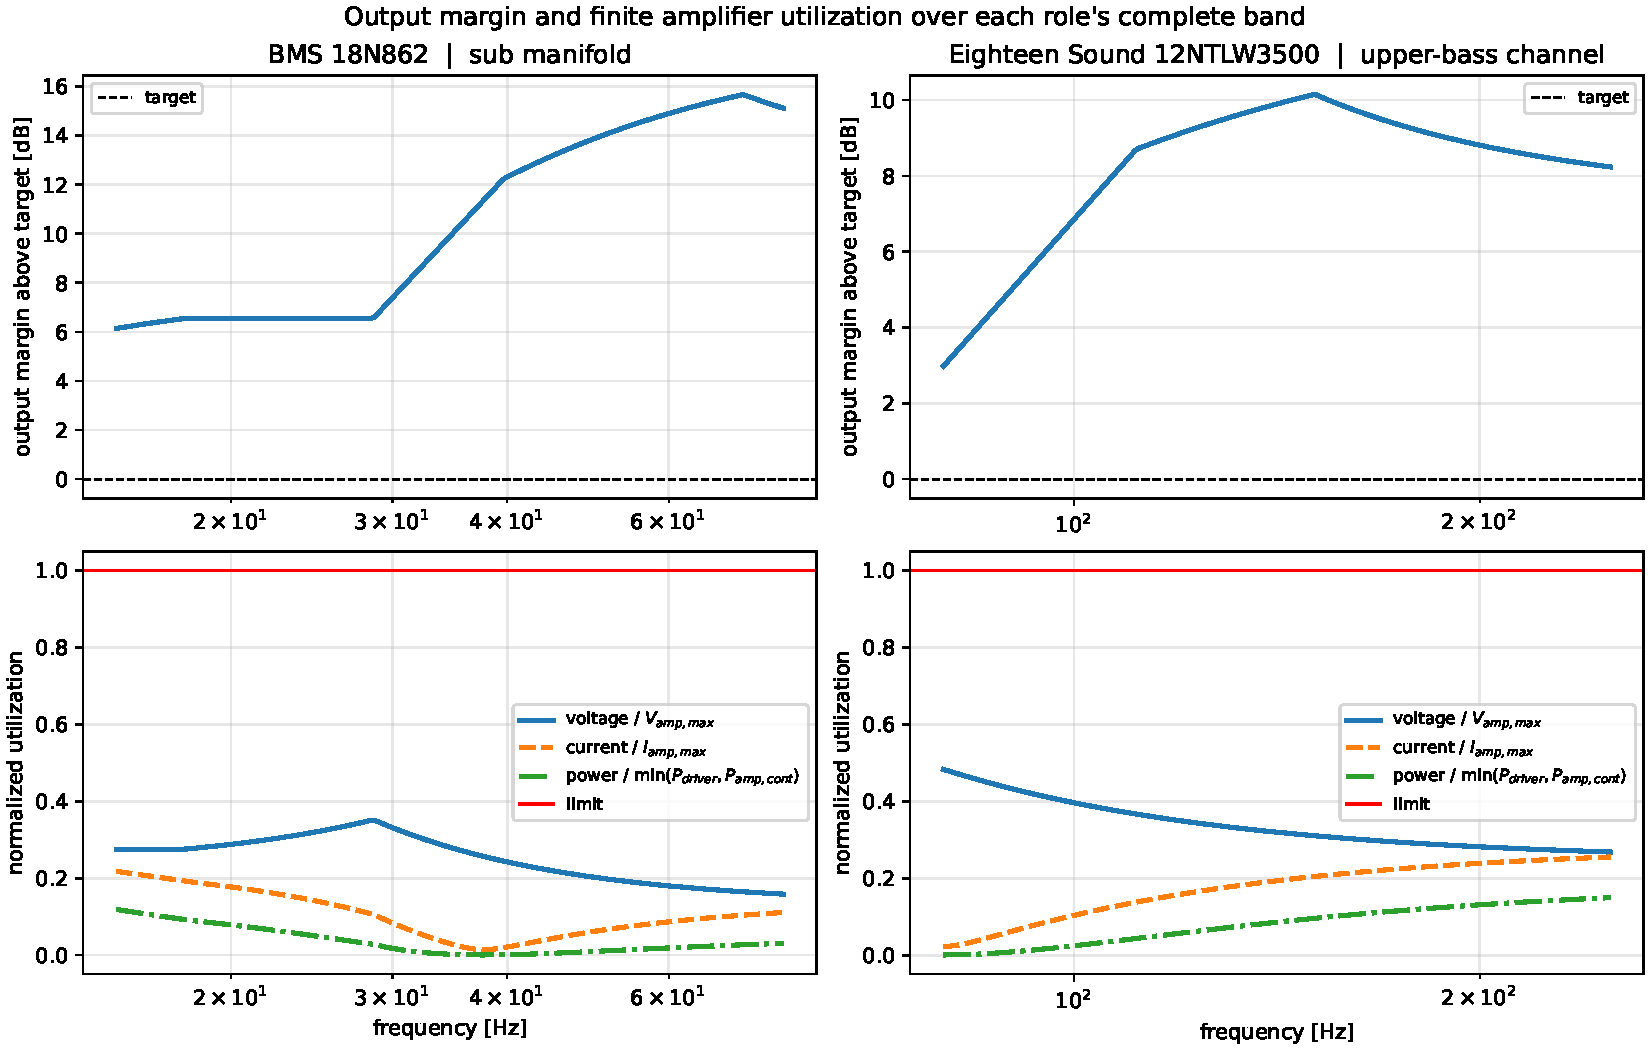
\includegraphics[width=\columnwidth]{../figures/fig_output_electrical}
	\caption{Output margin and finite amplifier utilization over each role's
	complete band, on one couch-area reference basis. Top: margin of the
	combined ceiling \cref{eq:master} above the role's target. Bottom:
	required rms voltage, current, and coil power per physical driver,
	\cref{eq:Ereq,eq:Ireq,eq:Preq}, normalized by the declared per-driver
	amplifier and driver limits. Left column: mono low-bass manifold; right
	column: one independent stereo upper-bass channel.}
	\label{fig:output-electrical}
\end{figure}
